\documentclass[border=5pt]{standalone}
\usepackage{pgfplots}
\pgfplotsset{compat=1.18}
\usepackage{siunitx}
\usepackage{tikz}
\usetikzlibrary{calc}

\definecolor{adam}{RGB}{31,119,180}
\definecolor{sgd}{RGB}{255,127,14}
\definecolor{rmsprop}{RGB}{143,0,255}

\begin{document}
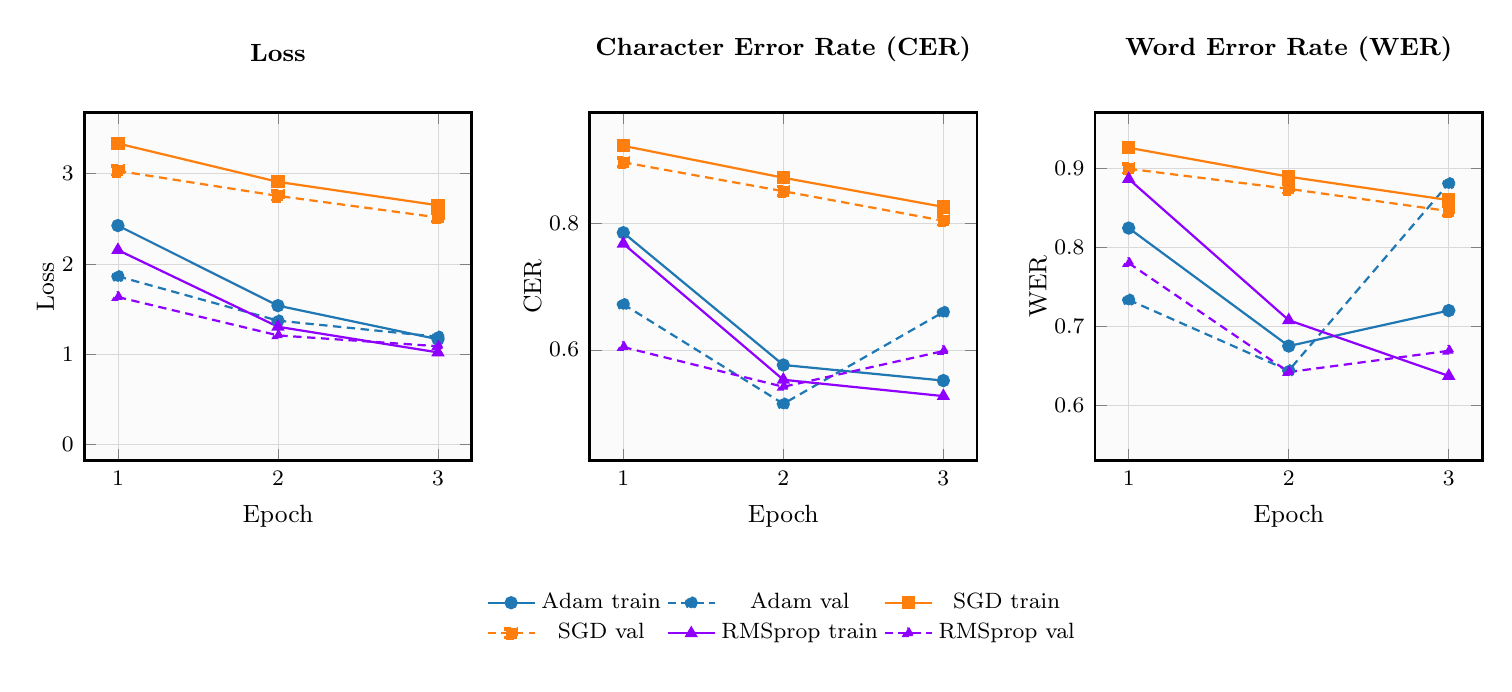
\begin{tikzpicture}[remember picture]

    % Графік 1: Loss
    \begin{axis}[
        name=plot1,
        width=6.5cm,
        height=6cm,
        xlabel={Epoch},
        ylabel={Loss},
        ylabel style={yshift=-0.15cm},
        xmin=0.9, xmax=3.1,
        ymin=0, ymax=3.5,
        xtick={1,2,3},
        grid=both,
        grid style={line width=.1pt, draw=gray!10},
        major grid style={line width=.2pt,draw=gray!30},
        title={Loss},
        axis background/.style={fill=gray!3},
        title style={yshift=3mm, font=\small\bfseries},
        label style={font=\small},
        tick label style={font=\footnotesize},
        line width=1pt,
        enlarge x limits=0.05,
        enlarge y limits=0.05,
        every axis plot/.append style={mark size=2pt},
        legend to name=commonlegend,
        legend columns=3,
        legend style={draw=none, fill=none, font=\footnotesize}
    ]
        % Adam
        \addplot[color=adam, mark=*, thick] coordinates {(1,2.4253) (2,1.5392) (3,1.1668)};
        \addplot[color=adam, mark=*, thick, densely dashed] coordinates {(1,1.8636) (2,1.3733) (3,1.1945)};
        
        % SGD
        \addplot[color=sgd, mark=square*, thick] coordinates {(1,3.3337) (2,2.9091) (3,2.6494)};
        \addplot[color=sgd, mark=square*, thick, densely dashed] coordinates {(1,3.0304) (2,2.7538) (3,2.5151)};
        
        % RMSprop
        \addplot[color=rmsprop, mark=triangle*, thick] coordinates {(1,2.1544) (2,1.3057) (3,1.0215)};
        \addplot[color=rmsprop, mark=triangle*, thick, densely dashed] coordinates {(1,1.6344) (2,1.2102) (3,1.0900)};
        
        \legend{Adam train, Adam val, SGD train, SGD val, RMSprop train, RMSprop val}
    \end{axis}
    
    % Графік 2: CER, розташовується праворуч від plot1
    \begin{axis}[
        name=plot2,
        at={($(plot1.east)+(1.5cm,0)$)},
        anchor=west,
        width=6.5cm,
        height=6cm,
        xlabel={Epoch},
        ylabel={CER},
        ylabel style={yshift=-0.15cm},
        xmin=0.9, xmax=3.1,
        ymin=0.45, ymax=0.95,
        xtick={1,2,3},
        grid=both,
        grid style={line width=.1pt, draw=gray!10},
        major grid style={line width=.2pt,draw=gray!30},
        title={Character Error Rate (CER)},
        axis background/.style={fill=gray!3},
        title style={yshift=3mm, font=\small\bfseries},
        label style={font=\small},
        tick label style={font=\footnotesize},
        line width=1pt,
        enlarge x limits=0.05,
        enlarge y limits=0.05,
        every axis plot/.append style={mark size=2pt}
    ]
        % Adam
        \addplot[color=adam, mark=*, thick] coordinates {(1,0.7852) (2,0.5761) (3,0.5514)};
        \addplot[color=adam, mark=*, thick, densely dashed] coordinates {(1,0.6721) (2,0.5147) (3,0.6598)};
        
        % SGD
        \addplot[color=sgd, mark=square*, thick] coordinates {(1,0.9225) (2,0.8721) (3,0.8260)};
        \addplot[color=sgd, mark=square*, thick, densely dashed] coordinates {(1,0.8965) (2,0.8508) (3,0.8041)};
        
        % RMSprop
        \addplot[color=rmsprop, mark=triangle*, thick] coordinates {(1,0.7678) (2,0.5527) (3,0.5269)};
        \addplot[color=rmsprop, mark=triangle*, thick, densely dashed] coordinates {(1,0.6044) (2,0.5416) (3,0.5981)};
    \end{axis}
    
    % Графік 3: WER, розташовується праворуч від plot2
    \begin{axis}[
        name=plot3,
        at={($(plot2.east)+(1.5cm,0)$)},
        anchor=west,
        width=6.5cm,
        height=6cm,
        xlabel={Epoch},
        ylabel={WER},
        ylabel style={yshift=-0.15cm},
        xmin=0.9, xmax=3.1,
        ymin=0.55, ymax=0.95,
        xtick={1,2,3},
        grid=both,
        grid style={line width=.1pt, draw=gray!10},
        major grid style={line width=.2pt,draw=gray!30},
        title={Word Error Rate (WER)},
        axis background/.style={fill=gray!3},
        title style={yshift=3mm, font=\small\bfseries},
        label style={font=\small},
        tick label style={font=\footnotesize},
        line width=1pt,
        enlarge x limits=0.05,
        enlarge y limits=0.05,
        every axis plot/.append style={mark size=2pt}
    ]
        % Adam
        \addplot[color=adam, mark=*, thick] coordinates {(1,0.8240) (2,0.6748) (3,0.7197)};
        \addplot[color=adam, mark=*, thick, densely dashed] coordinates {(1,0.7332) (2,0.6438) (3,0.8805)};
        
        % SGD
        \addplot[color=sgd, mark=square*, thick] coordinates {(1,0.9256) (2,0.8890) (3,0.8594)};
        \addplot[color=sgd, mark=square*, thick, densely dashed] coordinates {(1,0.8990) (2,0.8736) (3,0.8455)};
        
        % RMSprop
        \addplot[color=rmsprop, mark=triangle*, thick] coordinates {(1,0.8861) (2,0.7075) (3,0.6370)};
        \addplot[color=rmsprop, mark=triangle*, thick, densely dashed] coordinates {(1,0.7797) (2,0.6419) (3,0.6688)};
    \end{axis}

    % Розміщення загальної легенди під усіма графіками
    \node at ($(plot1.south)!0.5!(plot3.south)+(0,-2.0cm)$) {\pgfplotslegendfromname{commonlegend}};
    
\end{tikzpicture}
\end{document}